\begin{frame}[t]{Human auditory system}
\begin{itemize}
\item{Cocktail party effect}
\\Ability to keep your attention on only one voice even if there are many other people talking in the same time
\begin{center}
	\includegraphics[width=2.5in]{../pict/cocktail_party_effect}
\end{center}
\end{itemize}
\end{frame}

\begin{frame}[t]{Human auditory system}
\begin{itemize}
\item Binaural hearing $\rightarrow$ localization $\rightarrow$ segregation
\begin{center}
	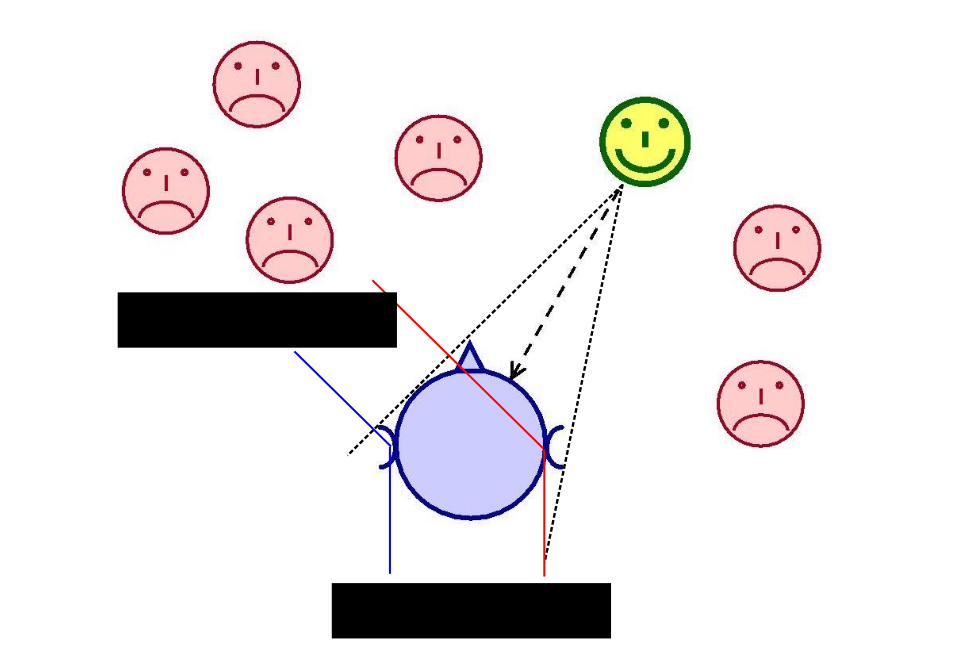
\includegraphics[scale=0.2]{../pict/CPP.png}
\end{center}
\end{itemize}
\end{frame}

\begin{frame}[t]{Human auditory system}
\begin{itemize}
\item Binaural hearing $\rightarrow$ localization $\rightarrow$ segregation
\begin{center}
	\includegraphics[scale=0.35]{../pict/cpp2.png}
\end{center}
\end{itemize}
\end{frame}

\begin{frame}[t]{Binaural Hearing}
\begin{itemize}
\item HRTF (head-related transfer function) both ear, 1.4 m, azimuth $0^o$ for a target and $5^o$, $10^o$, $20^o$, and $30^o$ for a masker.
\begin{center}
	\includegraphics[scale=0.6]{../pict/binaural_hearing.pdf}
\end{center}
\end{itemize}
\end{frame}

\begin{frame}[t]{Auditory Periphery}
\begin{itemize}
\item Gammatone-filter
	\begin{itemize}
	\item using $4^{th}$order gammatone-filter
	\begin{equation}\label{pers:gammatone}
	g(t) ~=~ at^{3}e^{-2\pi bt}\cos(2 \pi ft + \phi)
	\end{equation}
	\item with 128 center frequency distributed in scale ERB 80 Hz to 5000 Hz.
	\begin{equation}\label{pers:erb}
	ERB(f) ~=~ 24.7 \left( \frac{4.37 f}{1000} + 1\right)
	\end{equation}
	\end{itemize}
\item Middle ear gain: provides gain to simulate the effects of middle-ear function based on equal-loudness of BS3383, Normal Equal-Loudness Level.
\item Hair cells: model the activity of the auditory-nerve that represented by firing-probability in inner ear
\end{itemize}
\end{frame}

\begin{frame}[t]{Binaural Cue Extraction}
\begin{itemize}
\item Interaural time difference (ITD)
\begin{equation}\label{pers:itd}
C(i, j, \tau) ~=~ \frac{\sum_{k=0}^{K-1}(l_i(j-k)-\bar{l_i})(r_i(j-k-\tau)-\bar{r_i})}{\sqrt{\sum_{k=0}^{K-1}(l_i(j-k)-\bar{l_i})^2}\sqrt{\sum_{k=0}^{K-1}(r_i(j-k)-\bar{r_i})^2}}
\end{equation}
\item Interaural level difference (ILD)
\begin{equation}\label{pers:ild}
ILD_i = 20log_{10}\frac{\sum_i l_i^2(t)}{\sum_i r_i^2(t)}
\end{equation}
\end{itemize}
\end{frame}

\begin{frame}[t]{Relative Strength Estimation}
Energy ratio between target to masker signal
\begin{equation}
RS_i = \frac{\sum_i s_i^2(t)}{\left(\sum_i s_i^2(t) + \sum_i n_i^2(t)\right)}
\end{equation}
\end{frame}

\begin{frame}[t]{Probability Density Estimation}
\begin{itemize}
\item Patterns analysis between both ITD and ILD to the relative strength.
\item Probability density performed at the relative strength of two types:
	\begin{itemize}
	\item target signal is more dominant than a masker signal ($RS > 0.5$)
	\item masker signal are more dominant or equal than a target signal ($RS \leq 0.5$)
	\end{itemize}
\end{itemize}
\end{frame}

\begin{frame}[t]{Probability Density Estimation}
\begin{itemize}
\item{\scriptsize PDE for ITD and ILD to (a) relative strength ($RS \ge 0.5$) and (b) ($RS \leq 0.5$) of target and masker at $0^o$ and $30^o$ with SIR 10 dB and center frequency 500 Hz}
\begin{center}
	\includegraphics[scale=0.23]{../pict/pde-eps-converted-to.pdf}
\end{center}
\end{itemize}
\end{frame}
